\documentclass[10pt,a4paper]{article}
\usepackage[utf8]{inputenc}
\usepackage{marginnote}
\usepackage{algorithm}
\usepackage{algpseudocode}
\usepackage{graphicx}
\usepackage{caption}
\usepackage{subcaption}


\title{Clutter reduction in Parallel Coordinates using locality-aware clustering}
\author{An\v{z}e Stari\v{c} and Janez Dem\v{s}ar and Bla\v{z} Zupan}
\begin{document}
\maketitle
\section{Introduction}
Parallel coordinates are a way of presenting multivariate data in a 2D plot. It is a commonly used visualization, but does not scale well to large datasets (>1000 data points), as large number of lines results in too much visual clutter that obscures the trends we are looking for.

Several approaches have been proposed for reducing clutter. Most of them are based on aggregating data and later drawing the aggregates as densities~\cite{HW09}, wavelets~\cite{RZH12}, polygons~\cite{AA04, N04} or bars with varying opacity~\cite{BH03,FWR99b}.

Many authors~\cite{FWR99b,JLJC05,N04,AA04} use clustering as an aggregating function splitting data into multiple subsets and displaying properties of those subsets on the parallel coordinates plot. These methods usually use hierarchical~\cite{FWR99b} clustering when they need multiple levels of detail, or k-means clustering because of its speed. These clustering algorithms optimize clusters globally and do not care for the ordering of the features in the visualization.

We propose a novel clutter reducing technique using locality aware clustering. It is based on the Gaussian Mixture Models which are learned using expectation maximization. Learning process uses information about the order of attributes in the visualization to produce clusters that are optimized for the given projection. The resulting clusters have smaller variance and are better separated in the parallel coordinates plot than those obtained with the ordinary clustering methods.

\section{Related work}
Multiple existing methods use clustering to reduce clutter.

Fua et.al~\cite{FWR99b} use hierarchical clustering to provide multiple representations with different level of detail. Clusters are displayed as bands with opaque means and transparency linearly decreasing towards the cluster edge. This emphasizes the cluster width, but does not provide information about the examples within the cluster.

Johansson et. al~\cite{JLJC05} crate high-precision textures for clusters and outliers and combine those with transfer function to create visualizations. Changing the transfer function allows the user to put emphasis on different aspects of data. Different statistical properties of the data can be displayed using visualization.

Novotny~\cite{N04} uses a modified version of k-means clustering and displays clusters as polygons covering all examples in the cluster. Polygons are sorted by size before they are displayed to optimize the visibility of dense clusters.

Andrienko et. al~\cite{AA04} propose two methods of visualizing distribution of attribute values within clusters. First approach splits intersection of cluster with each axis into quantiles and then draws lines connecting them, thus showing dense parts as narrow bands within the cluster. Another approach are ellipse plots that can be shown behind each axis and also visualize axis value distribution.

Our approach is similar to~\cite{FWR99b,JLJC05,N04} as it also uses clusters to reduce clutter. Like~\cite{BH03}, it uses probability based clustering that assigns example a probability of belonging to a specific cluster. Clusters are drawn with polygon like in~\cite{N04,AA04}. We borrow drawing quantiles in clusters from~\cite{AA04} to provide additional information about value distribution inside clusters.

\section{Expectation maximization}
\marginnote{TODO: definicija preisana iz enega clanka, povzemi po svoje}
A Gaussian mixture model (GMM) is a parametric statistical model that assumes that the data originates from a weighted sum of several Gaussian sources. More formally, a GMM is given by
$p(x|\Theta) = \sum^k_{j=1}\alpha_jp(x|\theta_j)$, where $\alpha_j$ denotes the weight of each Gaussian, $\theta_j$ its respective parameters and  $k$ denotes the number of Gaussian sources in GMM. Expectation maximization (algorithmi~\ref{std_gmm}) is a widely used method for estimating parameter set of the model ($\Theta$) using unlabeled data~\cite{DLR77}. In the algorithms, we optimize GMM for dataset $X$, which has $m$ examples, and each of the Gaussians is parametrized by mean $\mu$, covariance matrix $\Sigma$ and its prior $\phi$. 


\begin{algorithm}
\caption{Standard EM GMM}
\label{std_gmm}
\begin{algorithmic}
\Function{em\_gmm}{$max\_steps$, $X$}
\State $initialize(\mu, \Sigma, \phi)$
\For {$step$   {\bf in} $1..max\_step$}
    \For {{\bf each} $i\gets1..m$, $j\gets1..k$}
        \State $w_j^{(i)}\gets p(z^{(i)} = j|x^{(i)}; \phi, \mu, \Sigma)$
    \EndFor
    \State
    \State $\phi_j\gets\frac{1}{m}\sum_{i=1}^{m}w_j^{(i)}$
    \State $\mu_j\gets\frac{\sum_{i=1}^mw_j^{(i)}x^{(i)}}{\sum_{i=1}^mw_j^{(i)}}$
    \State $\Sigma_j\gets\frac{\sum_{i=1}^mw_j^{(i)}(x^{(i)}-\mu_j)(x^{(i)}-\mu_j)^T}{\sum_{i=1}^mw_j^{(i)}}$
\EndFor
\EndFunction
\end{algorithmic}
\end{algorithm}

\section{Locality aware clustering}
\begin{figure}
		\label{fig:comparekm}
        \centering
        \begin{subfigure}[b]{0.45\textwidth}
                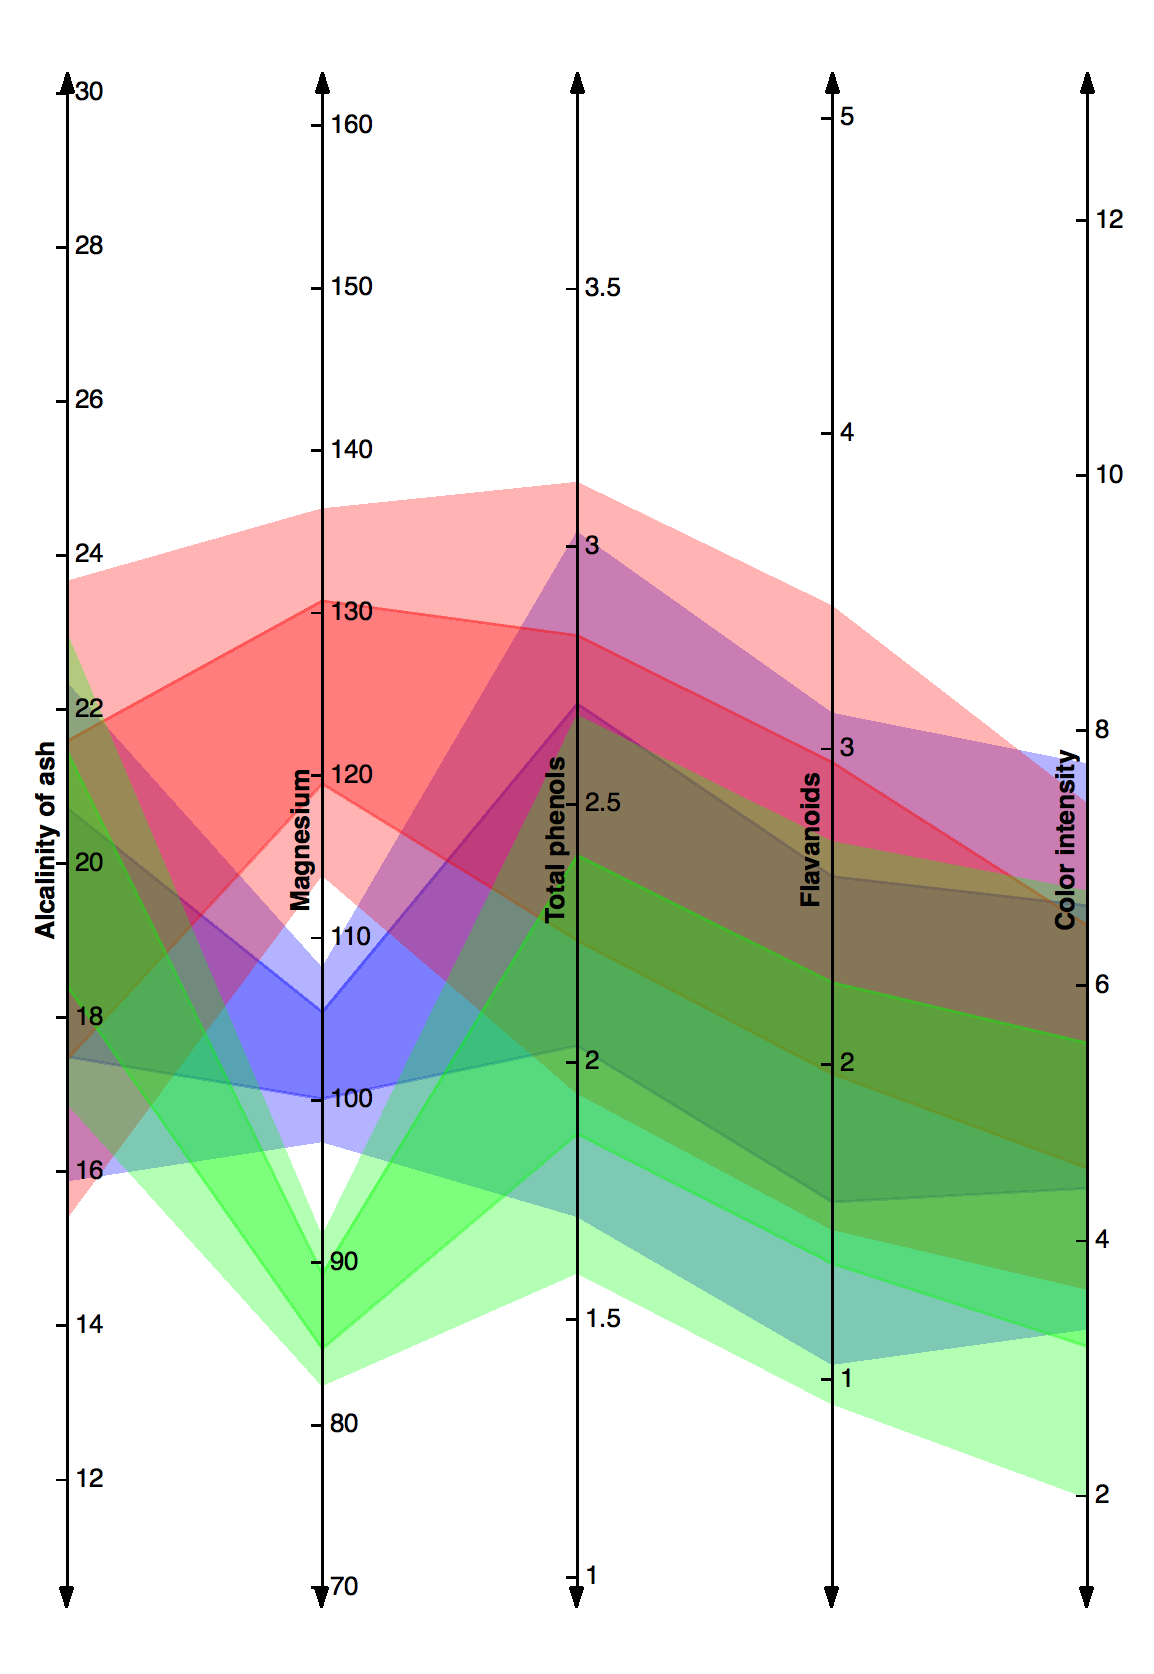
\includegraphics[width=\textwidth]{wine-kmeans}
                \caption{k-means clusters}
                \label{fig:winekm}
        \end{subfigure}%
        ~ %add desired spacing between images, e. g. ~, \quad, \qquad etc.
          %(or a blank line to force the subfigure onto a new line)
        \begin{subfigure}[b]{0.45\textwidth}
                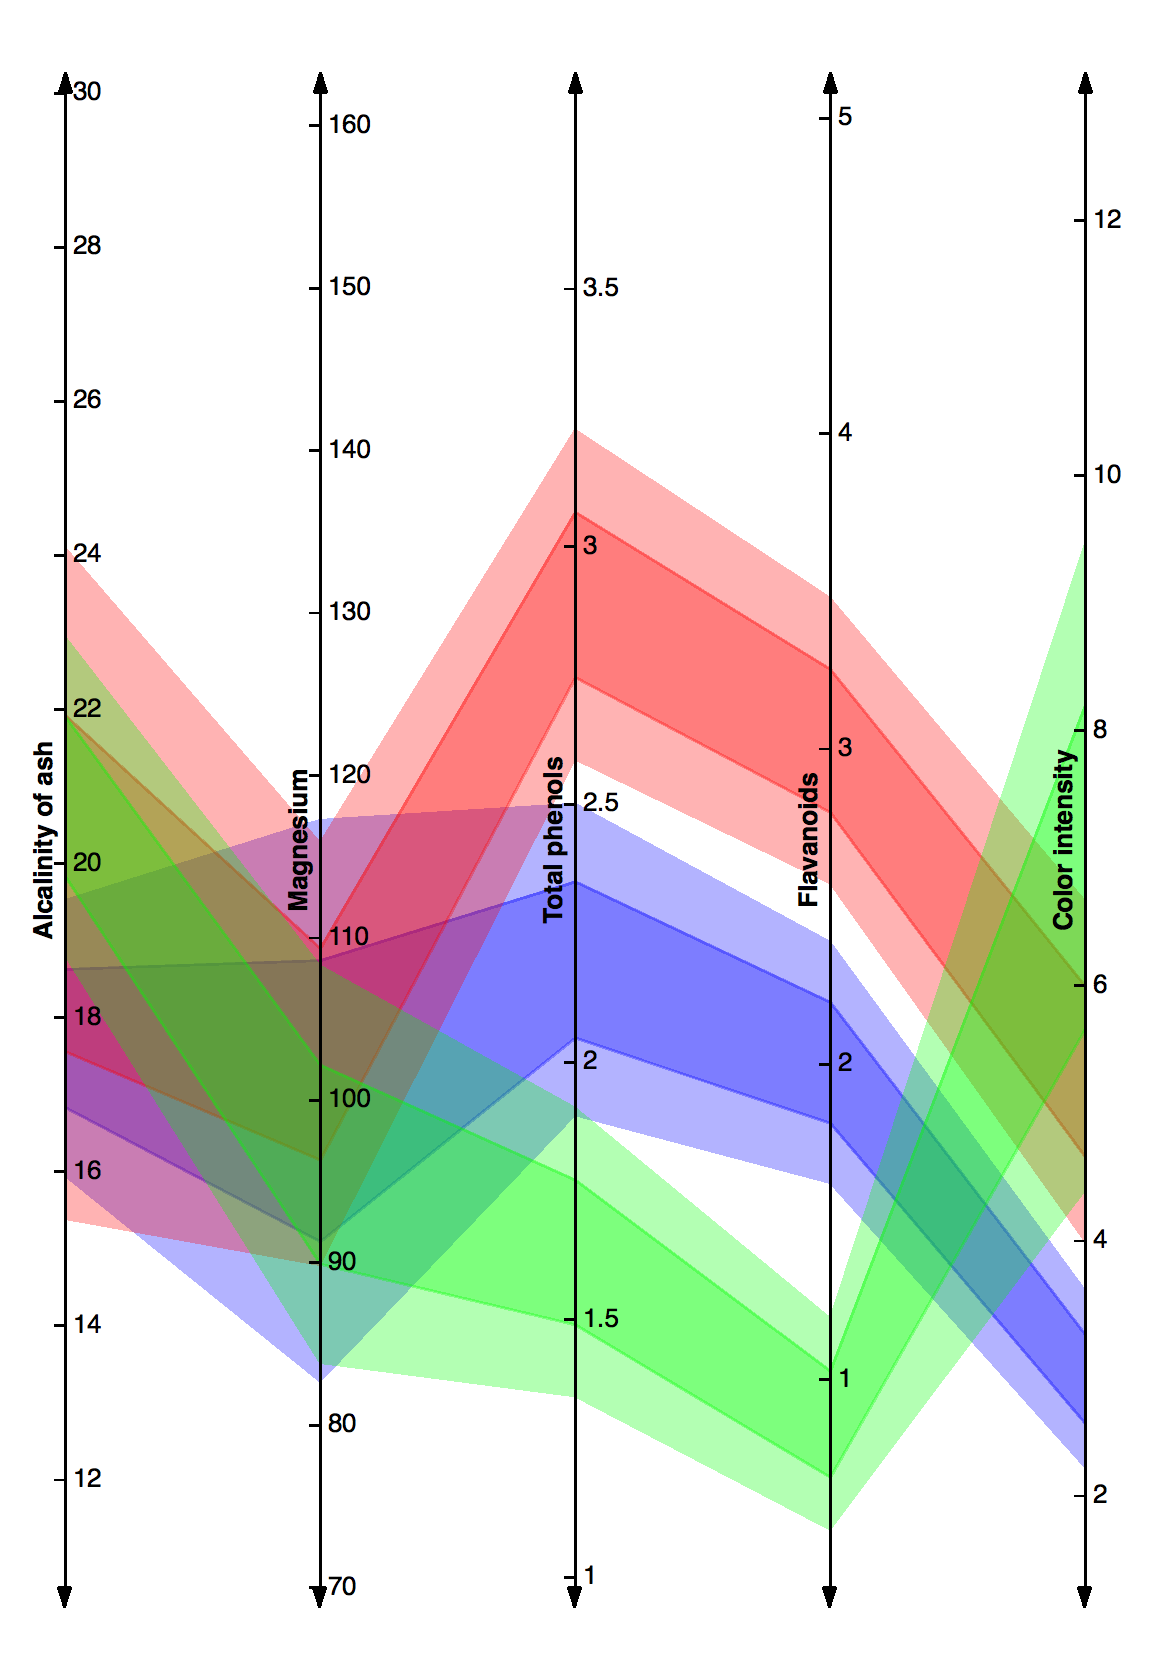
\includegraphics[width=\textwidth]{wine-la}
                \caption{locality aware clusters}
                \label{fig:winela}
        \end{subfigure}
        \caption{Comparison of clusters produced with k-means on the left (a) and locality aware clustering on the right (b). Our method finds clusters that are narrower and better separated in maximum number of axes.}\label{fig:animals}
\end{figure}

Learning a mixture of Gaussian models on multidimensional vectors constructs a model that takes all features into account. Clusters fit the data well, but when displayed on a parallel coordinates display they overlap.

Learning a mixture of Gaussians for each feature independently leads to clusters that fit value distribution for each feature well, but now examples that belong to the same cluster on one feature connect to multiple clusters on the other feature which results in noise.

Our method (algorithm~\ref{our_gmm}) optimizes each component of the parameters independently, but considers local neighborhood when calculating updates. When drawn on the parallel coordinates plot, computed clusters are better separated and produce less clutter compared to the clusters computed with k-means.
\begin{algorithm}
\caption{Modified EM GMM}
\label{our_gmm}
\begin{algorithmic}
\Function{our\_em\_gmm}{$max\_steps$, $window\_size$, $X$}
\State $initialize(\mu, \Sigma, \phi)$
\For {$step$   {\bf in} $1..max\_step$}
    \For {$f$ {\bf in} $features$}
        \State $XS\gets select\_features(f, window\_size, X)$
        \For {{\bf each} $i\gets1..m$, $j\gets1..k$}
            \State $w_j^{(i)}\gets p(z^{(i)} = j|xs^{(i)}; \phi, \mu, \Sigma)$
        \EndFor
        \State
        \State $\phi_{j}\gets\frac{1}{m}\sum_{i=1}^{m}w_j^{(i)}$
        \State $\mu_{j,f}\gets\frac{\sum_{i=1}^mw_j^{(i)}xs^{(i)}}{\sum_{i=1}^mw_j^{(i)}}$
        \State $\Sigma_{j,f}\gets\frac{\sum_{i=1}^mw_j^{(i)}(xs^{(i)}-\mu_j)(xs^{(i)}-\mu_j)^T}{\sum_{i=1}^mw_j^{(i)}}$
    \EndFor
\EndFor
\EndFunction
\end{algorithmic}
\end{algorithm}

\section{Evaluation}

\begin{thebibliography}{9}

\bibitem{AA04}
  G. Andrienko and N. Andrienko.
  Parallel coordinates for exploring properties of subsets.
  In \emph{Procedings of the Second International Conference on Coordinated and Multiple Views in Exploratory Visualizations} (2004),
  pp. 93-104.

\bibitem{BH03}
  M. Berthold and L. Hall.
  Visualizing fuzzy points in parallel coordinates.
  \emph{IEEE Transactions on Fuzzy Systems} 11(3), (2005),
  pp. 369-374.

\bibitem{DLR77}
  A. P. Dempster, N.M. Laird, and D.B. Rubin.
  \emph{Maximum likelihood from incomplete data via the EM algorithm}.
  JRSSB, 39:1-38,
  1997

\bibitem{FWR99b}
  Y. H. Fua, M. O. Ward and E. A. Rundensteiner.
  Hierarchical parallel coordinates for exploration of large datasets.
  In \emph {Proceedings of IEEE Visualization} (1999),
  pp. 43-50.
  
\bibitem{HW09}
  J. Heinrich and D. Weiskopf.
  Continuous parallel coordinates.
  \emph{IEEE Transactions on Visualization and Computer Graphics}, 15(6), (2009)
  pp. 1531-1538.
  
\bibitem{JLC07}
  J. Johansson, P. Ljung and  M. Cooper.
  Depth cues and density in temporal parallel coordinates.
  In \emph{Proceedings of the Eurographics/IEEE-VGTC Symposium on Visualization} (2007),
  pp. 35-42.
  
\bibitem{JLJC05}
  J. Johansson, P. Ljung, M. Jern and  M. Cooper.
  Revealing structure within clustered parallel coordinates displays.
  In \emph{Proceedings of the IEEE Symposium on Visualization} (2005),
  pp. 125-132.
  
\bibitem{NH06}
  M. Novotny and H. Hauser
  Outlier-preserving Focus+Context visualization in parallel coordinates.
  \emph{IEEE Transactions on Visualization and Computer Graphics}, 12(5), (2006),
  pp. 893-900.
  
\bibitem{N04}
  M. Novotny.
  Visually effective information visualization  of large data.
  In \emph{Proceedings of the 8th Central European Seminar on Computer Graphics} (2004),
  pp. 41-48.
  
\bibitem{RZH12}
  R. Rosenbaum, J. Zhi and B. Hamann.
  Progressive parallel coordinates,
  In \emph{Proceedings of the IEEE Pacific Visualization Symposium} (2012),
  pp. 25-32.
  

  


\end{thebibliography}

\end{document}